\subsection{Graphical User Interface}

%%Insert some paper citation that indicates user interfaces should be simple and blabla
%The User Interface provides the necessary information about the registered devices in a simple yet effective way;therefore, it is constituted by just two parts

The User Interface is constituted by two parts: the Main Window and the Configuration Dialog.

\subsubsection{Main Window}

The Main Window has two sections: the first allows the connection set-up with the panstamp server while the second displays the overall state of each entity in the network (see Figure ~\ref{java-server-main}). 

To establish a connection, the user has to select the serial port, which the panstamp is attached to, and the corresponding baud-rate. Once the connection is set up, the "connect" button is substituted by a "disconnect" button. The user can disconnect and connect the panstamp at any time. 
% For example if one decides to change the used seria port. 
If the Java server does not detect a device in any of the serial ports, the "connect" button will be unavailable (i.e. grayed out). To prevent the user from constantly restarting the server, we implemented a refresh button, which can be pressed at any time. When a device is finally detected, both options (connect and disconnect) will be available for that device.

The second section of the Main Window shows a table with the overall state of each entity in the network.
Among the data displayed are: the name of the entity's personality, the entity's status and a timestamp.
%explain each possible status (standby, idle, etc)
%explain what the timestamp is for
To reflect new detected entities in the network and changes in the entities' status, the information on the table is periodically updated; the table's refresh rate is configurable. 
%More information in the interface architecture section. %insert link here

\begin{figure}[h!]
 \centering
 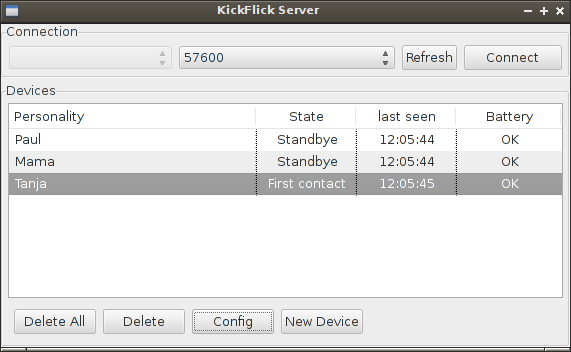
\includegraphics[width= 0.5\textwidth, clip=true  ,keepaspectratio=true]{./pic/java-server-main.png}
 % java-server-main.png: 0x0 pixel, 0dpi, nanxnan cm, bb=
 \caption{Main Window}
 \label{java-server-main}
\end{figure}

If the server detects an entity in the network, the user can select it in the device-table and open a configuration dialog by either pressing the configuration button (located on the bottom of the table) or double clicking on the intended table's item. A configuration dialog will then be opened where this particular device and its personality can be altered.

\subsubsection{Configuration Dialog}

The Configuration Dialog provides all the information about the selected entity's state and allows the configuration of the entity's personality. 

The user can customize a personality or select one among the predefined personalities. But if the user creates a personality and then selects a predefined one, all the changes made so far will be overridden by the predefined personality. 

To cancel all changes, the user has to click the ''close'' button located on the bottom-right corner of the Dialog Window (see Figure ~\ref{fig:java-server-config01}).   

In the Configuration Dialog, the personality's settings are distributed in 3 different tabs. The tab ''Basic'' (see Figure ~\ref{fig:java-server-config01}) contains the personality's name, the addresses of the two nodes that constitute the entity and a table with all the possible action keys. Only the checked keys will be enabled in the entity; that is, the entity will only react to a certain action key if the latter has a check next to it in the table. Every key can be enabled and disabled by the user. 


\begin{figure}[h!]
 \centering
 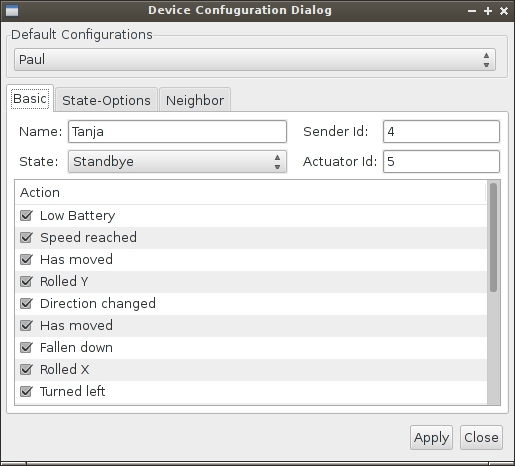
\includegraphics[width= 0.5\textwidth, clip=true  ,keepaspectratio=true]{./pic/java-server-config01.png}
 % java-server-main.png: 0x0 pixel, 0dpi, nanxnan cm, bb=
 \caption{Configuration Dialog, 1st Tab}
 \label{fig:java-server-config01}
\end{figure}

The ''State-Options'' tab shows in a checkbox the current state of the personality, which can be changed by the user. Below the checkbox, a table with all the personality's states is displayed. Here, the user can change the pattern and both colors of a particular state (see Figure ~\ref{fig:java-server-config02}). 


\begin{figure}[h!]
 \centering
 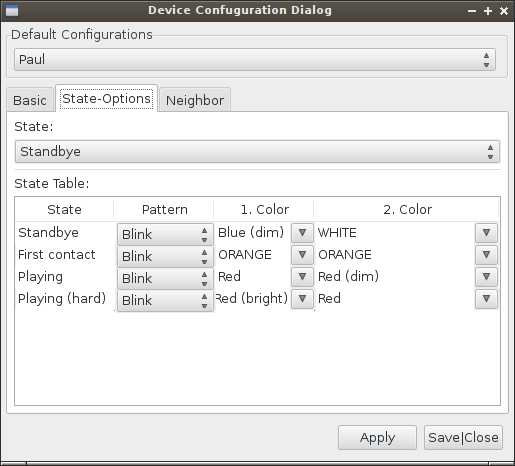
\includegraphics[width= 0.5\textwidth, clip=true  ,keepaspectratio=true]{./pic/java-server-config02.png}
 % java-server-main.png: 0x0 pixel, 0dpi, nanxnan cm, bb=
 \caption{Configuration Dialog, 2nd Tab}
 \label{fig:java-server-config02}
\end{figure}


Finally, the third tab labelled ''Neighbor'' displays the actions to be performed when the entity detects a neighbor (see Figure ~\ref{fig:java-server-config03}). The table shows the personality of each entity that has been detected by the server. However, if an entity has a preset personality, it will not be displayed in this tab since its reaction towards a neighbour is already defined and is not configurable. 

In this tab, the user can set the pattern and colors that the entity and its found neighbor will display. For instance, according to the settings in Figure ~\ref{fig:java-server-config03}, if the entity ''Mama'' finds ''Tanja'', both entities will exhibit a blink pattern with white and black. On the other hand, when ''Tanja'' finds ''Mama'', the two entities will again display a blink pattern but with different colors, namely red and blue. 

In order to save the changes made to the personality's settings, the user has to first press the ''apply'' and then the ''save|close'' button. Otherwise, if just the ''save|close'' button were pressed, no changes would be written and the device would keep the settings it had before the configuration process.

\begin{figure}[h!]
 \centering
 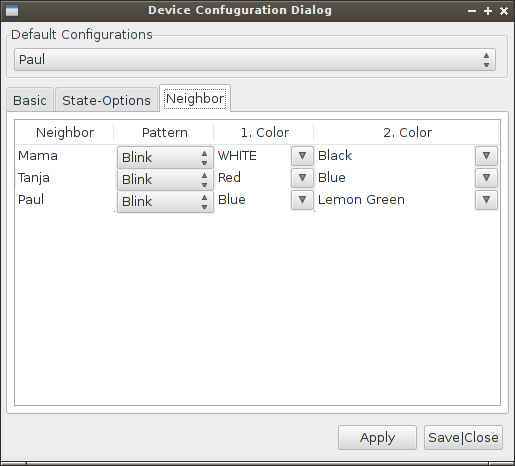
\includegraphics[width= 0.5\textwidth, clip=true  ,keepaspectratio=true]{./pic/java-server-config03.png}
 % java-server-main.png: 0x0 pixel, 0dpi, nanxnan cm, bb=
 \caption{Configuration Dialog, 3rd Tab}
 \label{fig:java-server-config03}
\end{figure}

\subsubsection{Interface Architecture}
The interface was created with the swt widget toolkit from eclipse. %insert cite
To periodically update the device table, the main window uses a swt timerevent. Every event-based action, like button clicks or selection were also implemented with the built-in event-listener structure of the swt toolkit. %insert cite again

When the dialog is opened, the entity will be passed as a parameter in the constructor, the dialog will then create the interface and afterwards read the entity's settings %Daniel, what do you mean by dialog here? The Configuration Dialog?

After changing one or more settings, if the user presses the ''apply'' button, these are kept in a temporal device. Then, if the ''save|close'' button is pressed, the new settings will be stored in a device instance that will be passed to the Main Window. When the user wants to discard the changes instead, he or she has to press the ''close'' button; the close action will pass a null pointer to the Main Window instance to indicate that no changes were committed. 

%The configuration will have no effect on the device at all, except the user says so. All changes will only be written when the apply button is pressed and even then a %temporally device will be created to first save all settings in the instance. If the user decides not to use the new settings and wants them to ignored, he then needs %to press the windows close button. The close action will pass a null pointer to the main window instance, signaling that no changes were commited.
%If, on the other hand, the user wants, after applying, to overwritte the device with the new settings he needs to close the configuration dialog by pressing the save %and close button. This will pass a device instance to the main window with all settings and therefor overwrite the previous settings of the device.

The Configuration Dialog widgets will be filled out on the creation of the dialog with all available data, e.g. reaction key names. After the interface is built, the device settings will be set. For example, this happens by setting the right selection for a combobox.
%I don't understand this paragraph :-(

The neighbor and state's tables are dynamically created; therefore, one can add more states and the number of possible neighbors is theoretically unlimited.


% vim: spell spelllang=en_gb 
